% !TEX root = ../ACT4E-ready.tex
\subsection{Monotone maps}
\AC{Add some motivation from design. E.g. generalization of "non-decreasing" and "non-increasing" from real numbers to partial orders}

\begin{definition}[Monotone map]
A \emph{monotone map} between posets~$\tup{A, \ordleq_A}$ and~$\tup{B, \ordleq_B}$ is a map that preserves the ordering, in the sense that 
\begin{equation}
 a \ordleq_A b \quad \Imp \quad f(a) \ordleq_B f(b).
\end{equation}

\begin{comment}\noindent A monotone map is an \emph{isomorphism} if the other direction
of the implication holds as well:
\begin{equation}
 a \leq_A b \quad \Leftrightarrow \quad f(a) \leq_B f(b).
\end{equation}
\end{comment}
\end{definition}
\begin{remark}
Given a poset~$A$,~$\id_A$ is monotone, since for~$a_1,a_2\in A$, one has:
\begin{equation}
\begin{aligned}
a_1\ordleq_A a_2 \Imp a_1&=a_1\then \id_A\\
&\ordleq_A a_2\then \id_A \\
&= a_2.
\end{aligned}
\end{equation}
\end{remark}

\begin{example}[Unit cost, total cost]
    \todo{Unit cost is antitone, total cost is monotone}
\end{example}

\begin{example}[Rounding functions]
    \todo{to write}
\end{example}


\begin{example}[Cardinality map]
In \cref{ex:hasseinclusion} we presented the poset arising from the power set of a set~$A=\{a,b,c\}$ and ordered via subset inclusion.

The map~$\vert \cdot \vert \colon \powerset(A)\to \mathbb{N}$ (cardinality), is a monotone map (\cref{fig:cardinality}).
\begin{figure}[h!]
\begin{center}
\includesag{40_dpcatfig_exmonotone}
\end{center}
\caption{The cardinality map is a monotone map. \label{fig:cardinality}}
\end{figure}
\end{example}

\begin{lemma}
Consider a discrete poset~$A$ and a poset~$B$. Any map~$f\colon A\to B$ is monotone.
\end{lemma}
\begin{proof}
Since~$A$ is a discrete poset, one has
\begin{equation}
    a_1\ordleq_A a_2 \iff a_1=a_2.
\end{equation}
Therefore, one has
\begin{equation}
\begin{aligned}
    a_1\ordleq_A a_2 &\Imp a_1=a_2\\
    &\Imp f(a_1)=f(a_2)\\
    &\Imp f(a_1)\ordleq_B f(a_2).
\end{aligned}
\end{equation}
\end{proof}
Unless indicated otherwise, in this paper all maps between posets are assumed to be monotone or will turn out to be monotone. In a similar way, one can define antitone maps.
\begin{definition}[Antitone map]
An \emph{antitone map} between two posets~$\tup{A, \ordleq_A}$ and~$\tup{B, \ordleq_B}$ is a map that reverses the ordering, in the sense that 
\begin{equation}
 a \ordleq_A b \quad \Imp \quad f(a) \ordgeq_B f(b).
\end{equation}
\end{definition}

\begin{example}
We now look at an example of \textbf{set-based filtering}, where filtering refers to online inference. Suppose that we want to track the value of a quantity~$x\in [0,100]$, without having a priory information about~$x$. We are equipped with sensors, which periodically measure the quantity~$x$ with some variable precision, i.e., at time~$t\in \mathbb{R}_{\geq 0}$ they produce an \emph{observation} $y_t\colon x_t\in [l_t,u_t]$. Also, note that the quantity fluctuates randomly, and we bound its ``velocity'' to be $\dot{x}_t\in [-1,1]$ (except at boundaries). At the beginning, our information state $\bar{i}_0$ could be that~$x\in [0,100]$. At time 0, we get an observation $y_0$, that says $x\in [21,24]$. The new information state can be obtained by ``fusing'' the two inputs we have received about~$x$. This corresponds to the intersection
\begin{equation*}
    x\in \left( [0,100] \cap [21,24]\right)\equiv x\in [21,24]
\end{equation*}
Let's now say we get an observation $y_1$ which says $x\in [19,22]$. We now need to take into account the evolution/dynamics of the quantity we are tracking. From the interval $[21,24]$ we know that the variable could have evolved in $[20,25]$ (dynamics are bounded with a unit increase/decrease). Therefore, the new information state is given by:
\begin{equation*}
    x\in \left( [20,25] \cap [21,24]\right)\equiv x\in [21,24]
\end{equation*}
One of the structures which could sustain this kind of inference, is the of \emph{posets of intervals}.
An interval is an ordered pair of elements~$\tup{l,u}$ of $P$, such that $l\ordleq_P u$. Given a poset~$P$, one can define a poset of intervals on~$P$. Intervals can be ordered by inclusion, e.g.:
\begin{equation*}
    \tup{l_1,u_1}\ordleq_{\mathrm{Int} P}\tup{l_2,u_2} \Leftrightarrow (l_1\ordleq_P l_2)\wedge (u_2\ordleq_P u_1).
\end{equation*}
The Hasse diagram representing a situation related to this diagram could be:
\begin{center}
    \begin{tikzcd}[column sep=tiny, row sep=tiny]
    x=1&&x=3&x=100\\
    &x\in[1,3]\arrow[dash,ul]\arrow[dash,ur]&&\\
    x\in[0,2]\arrow[dash,uu]&x\in [1,4]\arrow[dash,u] &&\\
    &x\in [0,4]\arrow[dash,u]\arrow[dash,ul]&&\\
    &&&x\in[0,100]\arrow[dash,ull]\arrow[dash,uuuu]
    \end{tikzcd}
\end{center}
\end{example}

\subsection{Compositionality of monotonicity}
Note that monotonicity is a compositional property.
\begin{lemma}
Given  posets~$A, B, C$ and monotone maps~$f\colon A \to B$ and~$g\colon B \to C$, the composite map~$f\then g\colon  A \to C$ is
monotone as well.
\end{lemma}
\begin{proof}
Consider~$a_1,a_2 \in A$,~$b_1,b_2\in B$. We have, by definition, 
\begin{equation}
\begin{aligned}
        a_1\ordleq_A a_2 &\Imp f(a_1)\ordleq_B f(a_2)\\ 
        b_1\ordleq_B b_2 &\Imp g(b_1)\ordleq_C g(b_2).
\end{aligned}
\end{equation}
By substituting the above in the map composition formula, one has
\begin{equation}
    a_1\ordleq_A a_2 \Imp (f\then g)(a_1) \ordleq_C (f\then g)(a_2),
\end{equation}
which is the monotonicity condition for~$(f\then g)$.
\end{proof}

\subsection{The category~\Pos of posets and monotone maps}
In this section, we want to abstract the concept of poset and describe a category in which the objects are posets themselves, and the morphisms are monotone functions between them. This category is called~$\Pos$.

\begin{definition}[Category \Pos]
    The category~$\Pos$ is defined by:
    \begin{compactenum}
    \item \emph{Objects}: The objects of this category are all posets.
    \item \emph{Morphisms}: The morphisms from a poset~$\Obja$ to a poset~$\Objb$ are the monotone maps from~$\Obja$ to~$\Objb$.
    \item \emph{Identity morphism}:  The identity morphism for the poset~$\Obja$
    is the identity map~$\id_\Obja$.
    \item \emph{Composition operation}: The composition operation is composition of maps.
    \end{compactenum}
\end{definition}

Occasionally we will write$f \colon \Obja \to_{\Pos} \Objb$ to emphasize that a monotone map between posets is a morphism in \Pos. Note that morphisms in \Pos are morphisms between posets, and posets are examples of categories. The notion of ``morphisms between categories'' is formally described by the notion of functor, which will be introduced later (\cref{def:functor}).

\subsection{Why~$\Pos$ is not sufficient for design theory}

The category \Pos of posets and monotone maps that we have described can model many facts that are useful for design theory. However, there are also limitations which motivate us to describe a more general category. This section describes the usefulness and the limitations of~$\Pos$.

\begin{example}[Battery]
Consider a model of a battery where the capacity is the functionality and the mass of the battery is the resource.
%(\cref{fig:battery-example}). 
There is certainly a monotone map from capacity to mass. This map answers the question: ``Given a value of the capacity, what is the minimum mass needed?''. Conversely, in the other direction, the map that answers the question: ``Given a certain mass, what is the maximum capacity that can be provided?'' is also a monotone map.
\end{example}

\begin{comment}
\begin{figure}[h!]
    \centering
    \begin{tikzcd}
    \bullet &\arrow[l] \bullet\\[-15pt]
    \text{mass} & \text{capacity}
    \end{tikzcd}
    \caption{Example of the design of a battery. \label{fig:battery-example}}
\end{figure}
\end{comment}

Therefore, at first sight it might seem that posets and monotone maps would be sufficient to describe a quantitative theory of design. However, there are more general relations to be modeled. It is easy enough to describe examples in which having a simple monotone map from functionality to resources is not sufficient.

\begin{example}[Delivery drone]
Consider the design of a delivery drone, in which the functional requirement is that the drone should be able to make a delivery at a distance~$d$ and we need to reason about how powerful to make the drone. In particular, we need to choose at what (average) \emph{velocity}~$v$ the drone  should travel and what is the optimal \emph{mission duration}. The relation between distance~$d$, velocity~$v$, and mission duration~$T$ is given by~$d=v\cdot T$. We can choose to have either a fast drone and short missions, or a slow drone and long missions. This is an interesting trade-off. Flying fast takes more energy, both for propulsion as well as for computation (more objects to be observed and processed). Flying too slow will also be excessively energy-consuming because of the long mission duration.

If we consider~$v$ and~$T$ as given, then the map~$\tup{v,T} \mapsto v\cdot T$ is clearly a monotone function that gives the distance which the drone can cover. However, in the other direction, we do not have a simple map, but rather a 1-to-many relation $\mathrm{distance}\to \mathrm{velocity}\times \mathrm{time}$. For each fixed value of the distance, there is an entire continuum of values of~$v$ and~$T$ which we can choose, as it can be seen in~\cref{fig:drone-example-antichain}.

\begin{figure}[h!]
    \centering
    % \includegraphics[scale=0.33]{dpcatfig_e2}
    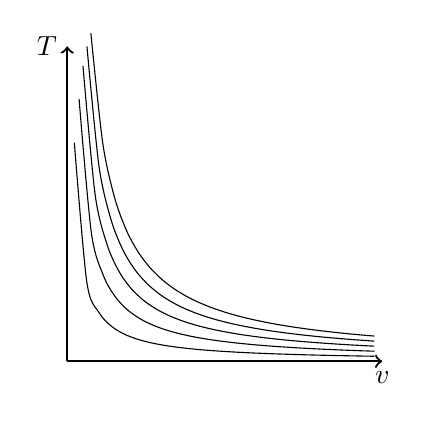
\begin{tikzpicture}
\draw[->, thick] (0,0)--(4,0) node[below]{$v$};
\draw[->, thick] (0,0)--(0,4) node[left]{$T$};
\draw[domain=0.3:3.9,smooth,variable=\t]plot (\t,1.25/\t);
\draw[domain=0.25:3.9,smooth,variable=\t]plot (\t,1/\t);
\draw[domain=0.2:3.9,smooth,variable=\t]plot (\t,0.75/\t);
\draw[domain=0.15:3.9,smooth,variable=\t]plot (\t,0.5/\t);
\draw[domain=0.09:3.9,smooth,variable=\t]plot (\t,0.25/\t);
\end{tikzpicture}
    \caption{Antichains in~$\tup{v,T}$ for different values of~$d$. \label{fig:drone-example}
    \label{fig:drone-example-antichain}}
\end{figure}

\end{example}

In other words, using~$\Cat{Pos}$ it is not possible to make a theory of \emph{trade-offs}. We will introduce a more general category, called  the category~$\Cat{DP}$ of \emph{design problems} (\cref{sec:dpdefinition}), which will allow to describe such a theory.

\GZ{Check with JL what he means}

\subsection{From antichains to uppersets, and viceversa}
\begin{definition}[Upper closure operator]
\label{def:upperclosure}
The \emph{upper closure operator} $\uparrow$ maps a subset to the smallest upper set that includes it, i.e.:
\begin{equation}
    \begin{aligned}
    \uparrow \colon \powerset(P)&\to \mathsf{U}P\\
    S&\mapsto \{y\in P \mid \exists x\in S \colon x\ordleq y\}.
    \end{aligned}
\end{equation}
\end{definition}
\begin{remark}
Note that, by definition, an upper set is closed to upper closure.
\end{remark}
\begin{remark}
For any~$S\in \powerset(P)$,~$\uparrow S$ is in fact an upper set.
\begin{proof}
Suppose~$y\in \uparrow S$ and~$z\in P$, and suppose $y\ordleq z$. By definition~$\exists x$ s.t.~$x\ordleq y$, meaning that~$x\ordleq z$. Thus,~$z\in \uparrow S$, as was to be shown.
\end{proof}
\end{remark}

\begin{lemma}
The upper closure operator~$\uparrow$ is a monotone map.
\end{lemma}
\begin{proof}
Consider the posets~$\tup{\powerset(P),\subseteq}$ and~$\tup{\mathsf{U}P,\supseteq}$, and~$S_1,S_2\in \powerset(P)$. It is clear that given~$S_1\subseteq S_2$, one has
\begin{equation}
    \{y\in P\mid \exists x\in S_1\colon x\ordleq y\} \supseteq \{y\in P\mid \exists x\in S_2\colon x\ordleq y\}.
\end{equation}
Therefore,~$\uparrow S_1\supseteq \ \uparrow S_2$, satisfing the monotonicity property for~$\uparrow$.
\end{proof}

\begin{lemma}\label{up-cl-inj-antichains}
Let $A$ and $B$ be subsets of $P$ that are antichains. Then
\begin{equation}
\uparrow A = \ \uparrow B \quad \Rightarrow \quad A = B.
\end{equation}
\end{lemma}

\begin{proof}
First, let's fix an $a \in A$. From $\uparrow A = \ \uparrow B$ we know that in particular $A \subseteq \ \uparrow B$. This means that for our fixed $a \in A$ there exists $b \in B$ such that $b \leq a$. From $\uparrow A = \ \uparrow B$ it also follows that $B \subseteq \ \uparrow A$, so to the  $b \in B$ given above, there exists $a' \in A$ such that $a' \leq b$. In total, we have $a' \leq b \leq a$, and since $A$ is an antichain, we must have $a' = a$. This implies that $a' = b = a$. In particular, we have $a \in B$. 

The above shows that $A \subseteq B$. To show $B \subseteq A$, we can fix any $b \in B$ and repeat the above argumentation, now with the roles of $A$ and $B$ exchanged.  
\end{proof}

In the example of the pizza recipes, first, consider the upper set of a single element of the poset, e.g.~$p_1=\tup{\unit[1]{USD},\unit[2]{h}}$  (\cref{fig:upperclosure_1}).
\begin{figure}[h!]
\begin{center}
\includesag{70_upper_closure_1}
\end{center}
\caption{The upper closure of a singleton set of pizza recipes. \label{fig:upperclosure_1}}
\end{figure}
Then, consider the case of two elements, with~$p_2=\tup{\unit[2]{USD},\unit[1]{h}}$ (\cref{fig:upperclosure_2}).

\begin{figure}[h!]
\begin{center}
    \includesag{70_upper_closure_2}
\end{center}
\caption{The upper closure of a set of pizza recipes. \label{fig:upperclosure_2}}
\end{figure}
Note that the upper set of the subset formed by the two elements is the union of the upper sets of the single elements.

\begin{definition}[Lower closure operator]
The \emph{lower closure operator} $\downarrow$ maps a subset to the smallest lower set that includes it, i.e.
\begin{equation}
    \begin{aligned}
    \downarrow\colon \powerset(P)&\to \mathsf{L}P\\
    S&\mapsto \{ y\in P \mid \exists x\in S \colon y\ordleq x\}.
    \end{aligned}
\end{equation}
\end{definition}

\begin{lemma}
The lower closure operator $\downarrow$ is a monotone map.
\end{lemma}

\JL{The following proof is a bit redundant... we can say ``analogous to the case of the upper closure operation'' and/or invoke the principle of duality for posets.}
\begin{proof}
Consider the posets~$\tup{\powerset(P),\subseteq}$ and~$\tup{\mathsf{L}P,\subseteq}$, and let~$S_1,S_2\in \powerset(P)$. It is clear that given~$S_1\subseteq S_2$, one has
\begin{equation}
    \{y\in P\mid \exists x\in S_1\colon y\ordleq x\} \subseteq \{y\in P\mid \exists x\in S_2\colon y\ordleq x\}.
\end{equation}
Therefore,~$\uparrow S_1\subseteq \ \uparrow S_2$, satisfing the monotonicity property for~$\downarrow$.
\end{proof}



\begin{example}
Consider the battery example of~\cref{ex:battery}, and the antichain given by the battery models~$a=\tup{\unit[10]{USD},\unit[1]{kg}}$,~$b=\tup{\unit[20]{USD},\unit[0.5]{kg}}$, and~$c=\tup{\unit[30]{USD},\unit[0.25]{kg}}$ (\cref{fig:examplebatt}).
The lower closure uperator~$\downarrow\{a,b,c\}$ represents all the battery models which, if existing, would dominate~$\{a,b,c\}$.

\end{example}
\begin{figure}[h!]
    \begin{center}
        \includesag{70_battery_1}
    \end{center}
    \caption{Battery example. From the left: antichain, upper closure, and lower closure.
        \label{fig:examplebatt}}
\end{figure}


\begin{definition}[Min]
\label{def:Min}
$\Min \colon \powerset(P) \to \antichains P$ is the map that sends a subset~$S$ of a poset to the minimal elements of that subset, i.e., those elements~$a \in S$ such that~$a \ordleq b$ for all~$b \in S$. In formulas:
\begin{equation}
    \begin{aligned}
    \Min \colon \powerset(P) &\to \antichains P\\
    S&\mapsto \{ x\in S\colon (y\in S)\wedge(y\ordleq x)\Rightarrow (x=y)\}.
    \end{aligned}
\end{equation}
Note that~$\Min(S)$ could be empty.
\end{definition}

\begin{definition}[Max]
\label{def:Max}
$\Max \colon \powerset(P) \to \antichains P$ is the map that sends a subset~$S$ of a poset to the maximal elements of that subset, i.e., those elements~$a \in S$ such that~$a \ordgeq b$ for all~$b \in S$. In formulas:
\begin{equation}
    \begin{aligned}
    \Max \colon \powerset(P) &\to \antichains P\\
    S&\mapsto \{ x\in S\colon (y\in S)\wedge(y\ordgeq x)\Rightarrow (x=y)\}.
    \end{aligned}
\end{equation}
Note that~$\Max(S)$ could be empty.
\end{definition}

\todo{This is a remnant of older times. To remove. }

\begin{lemma}
Given a poset~$\tup{P,\ordleq}$,~$\tup{\antichains P,\ordleq_{\antichains P}}$ is a poset with
\begin{equation}
\label{eq:orderantichain}
    A\ordleq_{\antichains P} B \text{ if and only if } \uparrow A \supseteq \ \uparrow B.
\end{equation}
Furthermore, it is bounded by the top~$\top_{\antichains P}=\emptyset$ and the bottom~$\bot_{\antichains P}=\{\bot_P\}$.
\end{lemma}

\begin{proof}
We need to show the poset properties (\cref{def:poset}).
We can prove the following:

\

\begin{compactitem}
\item \emph{Reflexivity}: From~$\tup{P,\ordleq}$ being a poset we know that 
\begin{equation}
\begin{aligned}
\{y\in P \mid \exists x\in A \colon x\ordleq y\} &\supseteq \{y\in P \mid \exists x\in A \colon x\ordleq y\},\\
\uparrow A =\ \uparrow A
\end{aligned}
\end{equation}
and hence~$A\ordleq_{\antichains P}A$.

\

\item \emph{Antisymmetry}: One has
\begin{equation}
    \begin{aligned}
    \left(A\ordleq_{\antichains P} B\right) \wedge \left(B\ordleq_{\antichains P} A\right)
    &\Leftrightarrow \left(\uparrow A \supseteq \ \uparrow \ B\right) \wedge \left( \uparrow  B\supseteq \ \uparrow \ A\right)\\
    &\Leftrightarrow \ \uparrow A= \ \uparrow B \\
    & \Rightarrow A = B.
    \end{aligned}
\end{equation}
The last implication is by Lemma \ref{up-cl-inj-antichains}. 

\


\item \emph{Transitivity}: One has
\begin{equation}
    \begin{aligned}
    \left(A\ordleq_{\antichains P} B\right) \wedge \left(B\ordleq_{\antichains P} C\right)&\Leftrightarrow  \left(\uparrow A \supseteq \ \uparrow \ B\right) \wedge \left( \uparrow  B\supseteq \ \uparrow C\right)\\
    &\Imp \ \uparrow A\supseteq \ \uparrow C\\
    &\Imp A\ordleq_{\antichains P}C.
    \end{aligned}
\end{equation}
In order to find the top, we need to find the smallest set~$\top_{\antichains P}$ such that~$A\ordleq_{\antichains P} \top_{\antichains P}$ for all~$A\in \antichains P$. In other words, such that~$\uparrow A\supseteq \ \uparrow \top_{\antichains P}$ for all~$A\in \antichains P$. This is clearly~$\emptyset$, since~$\uparrow \emptyset = \emptyset$. Similarly, in order to find the bottom, we need to find the set~$\bot_{\antichains P}$ such that~$\bot_{\antichains P} \ordleq_{\antichains P} A$ for all~$A\in \antichains P$. In other words, such that~$\uparrow \bot_{\antichains P} \supseteq \ \uparrow A$ for all~$A\in \antichains P$. We obtain a bottom if we set $\bot_{\antichains P} := \top_P$, since $\top_P \supseteq A$ for all $A \subseteq P$, and hence, by monotonicty of $\uparrow$, we have in particular $\uparrow \top_P \supseteq \ \uparrow A$ for all antichains $A$. 
\end{compactitem}
\end{proof}



\begin{definition}[Downward closed set]
\label{def:downward-closed-upperset}
An upper set~$S$ is \emph{downward-closed} in a poset~$P$ if
\begin{equation}
    S =\, \uparrow \Min S.
\end{equation}
\end{definition}

\begin{remark}
The set of downward-closed upper sets of~$P$ is denoted~$\underline{\mathsf{U}}P$.
\end{remark}


    
